\section{Pipeline Overview}

\subsection{Shared Processing Pipeline}

All three experiments follow a \textbf{unified data and training pipeline}, ensuring that any performance differences can be attributed to model architecture alone. The shared components are:

\begin{itemize}
    \item \textbf{Tokenizer:} \texttt{distilbert/distilbert-base-uncased} (all models receive identical token sequences).
    \item \textbf{Data splits:} Identical stratified train/val/test partitions (seed 42).
    \item \textbf{Loss function:} Cross-entropy over five classes.
    \item \textbf{Optimizer family:} AdamW for all experiments.
    \item \textbf{Checkpoint rule:} Best model saved when validation macro-F1 improves.
    \item \textbf{Early stopping:} Patience of 3 epochs on validation macro-F1.
    \item \textbf{Evaluation protocol:} Validation after every epoch; test evaluated once at the end using the best checkpoint.
    \item \textbf{Metrics:} Accuracy, macro-precision, macro-recall, macro-F1, per-class F1, confusion matrix.
\end{itemize}

\subsection{Pipeline Stages}

The end-to-end pipeline proceeds through five sequential stages, as illustrated in Figure~\ref{fig:pipeline}:

\begin{enumerate}
    \item \textbf{Data loading:} Raw CSV files are read; tweet text and sentiment labels are extracted. Labels are mapped to integer indices.
    \item \textbf{Splitting:} The official training file is split 90/10 (stratified) into train and validation subsets.
    \item \textbf{Tokenisation:} The shared DistilBERT tokenizer converts raw text to token IDs and attention masks with dynamic batch padding.
    \item \textbf{Model training:} Each experiment initialises its own model (EXP-1, EXP-2, or EXP-3), trains for up to the maximum number of epochs with early stopping, and saves the best checkpoint.
    \item \textbf{Evaluation:} The best checkpoint is loaded; predictions are computed on the held-out test set; metrics and visualisations are generated.
\end{enumerate}

\begin{figure}[H]
    \centering
    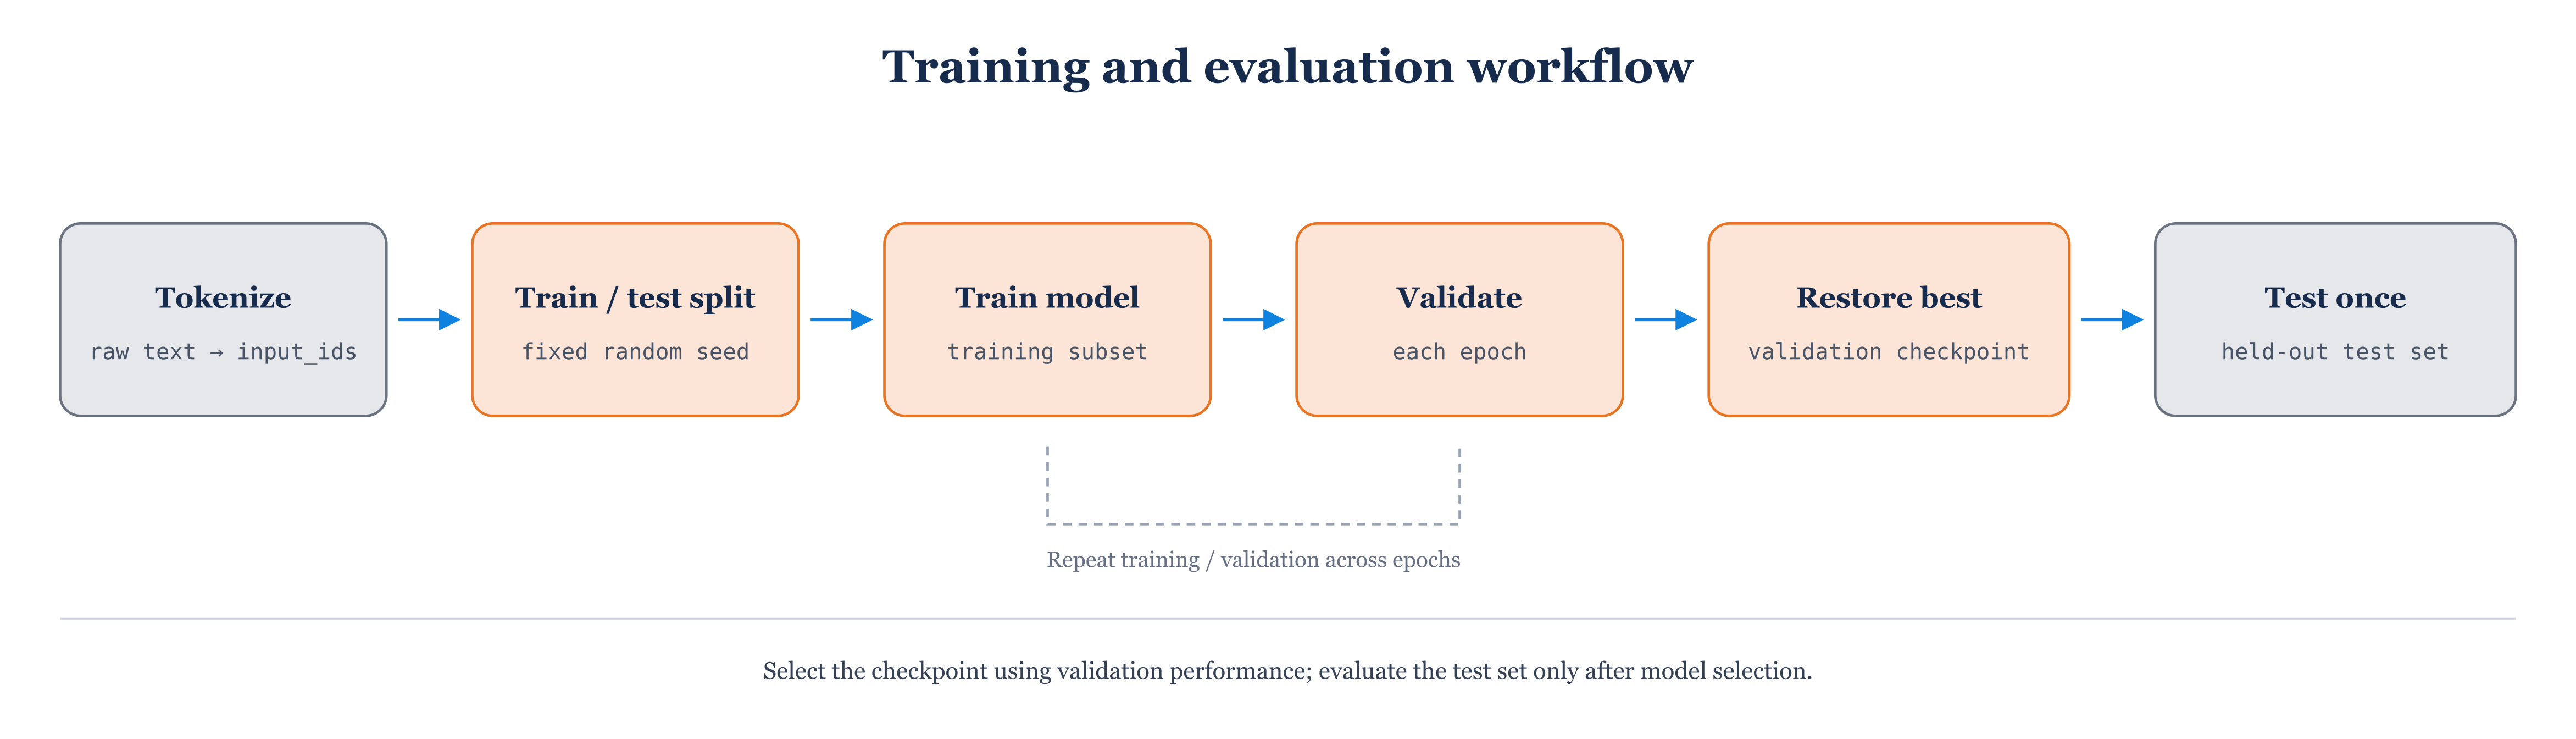
\includegraphics[width=\textwidth]{../../Assignment2/diagram-pipeline/pipeline-dl2.drawio.png}
    \caption{End-to-end pipeline shared by all three experiments (EXP-1 BiLSTM, EXP-2 DistilBERT frozen, EXP-3 DistilBERT full fine-tune).}
    \label{fig:pipeline}
\end{figure}

\subsection{Code Organisation}

The implementation is structured into the following modules within \path{Assignment2/code/}:

\begin{itemize}
    \item \textbf{\path{dataset.py}} — Dataset class (\texttt{TweetDataset}), tokenisation, \texttt{DataCollatorWithPadding}, and the \texttt{get\_dataloaders()} factory function.
    \item \textbf{\path{baseline\_model.py}} — All three model classes: \texttt{BiLSTMClassifier}, \texttt{DistilBertClassifier}.
    \item \textbf{\path{main.py}} — Training loop, validation loop, early stopping logic, checkpoint saving, test evaluation, and CLI argument parsing (\texttt{--base}, \texttt{--pretrained}, \texttt{--pretrained-frozen}).
    \item \textbf{\path{metrics.py}} — Metric computation (accuracy, macro-P/R/F1, per-class report, confusion matrix, FLOPs estimation, inference timing).
    \item \textbf{\path{plotter.py}} — Learning curve plots, confusion matrix heatmaps, dimensionality reduction visualisations (PCA, t-SNE, UMAP), class similarity matrices, and qualitative prediction grids.
    \item \textbf{\path{EDA.py}} — Standalone EDA script for class distribution, length statistics, temporal analysis, and duplicate detection.
\end{itemize}
